% =========================================================================
% Revised manuscript (v2) -- prepared after rejection from J. Comput. Electron.
% (Submission 5183a3bb-4b2c-4307-a79b-1faa62340b74). All numbers in this file are
% generated by ../src_v2 and stored in ../data_v2; see the response letter for the
% mapping between reviewer comments and changes.
% =========================================================================
\documentclass[11pt]{article}
\usepackage[utf8]{inputenc}
\usepackage[T1]{fontenc}
\usepackage{amsmath,amssymb}
\IfFileExists{mathdesign.sty}{\usepackage[bitstream-charter]{mathdesign}}{\usepackage{lmodern}}
\usepackage{booktabs}
\usepackage{graphicx}
\usepackage[margin=1in]{geometry}
\usepackage{xcolor}
\usepackage[colorlinks,linkcolor={red!50!black},citecolor={blue!50!black},urlcolor={blue!80!black}]{hyperref}
\usepackage{lineno}
\usepackage[english]{babel}
\urlstyle{same}
\providecommand{\doi}[1]{\href{https://doi.org/#1}{doi:\,#1}}
\DeclareSymbolFont{usualmathcal}{OMS}{cmsy}{m}{n}
\DeclareSymbolFontAlphabet{\mathcal}{usualmathcal}
\graphicspath{{../figures_v2/}}
\newcommand{\ohmcm}{\ensuremath{\Omega\cdot\mathrm{cm}}}

\title{Hole Injection at Top and Edge Metal Contacts to Few-Layer InSe:\\ A Verified Drift-Diffusion and Electro-Thermal Simulation Study}
\author{Harsha Adhikary\thanks{Corresponding author. Email: \href{mailto:harshaa@iisc.ac.in}{harshaa@iisc.ac.in}} \\[4pt]
\small Department of Physics, Indian Institute of Science (IISc), Bengaluru, India}
\date{}

\sloppy
\begin{document}
\maketitle

\begin{abstract}
\noindent
Efficient hole injection is the less-studied half of complementary logic in indium selenide (InSe). We simulate hole transport through 5-nm $\gamma$-InSe channels contacted by top (out-of-plane) and edge (in-plane) metal electrodes with an open-source DEVSIM model that couples Poisson's equation to the non-equilibrium carrier densities, uses a flux-balanced thermionic/thermionic-field-emission contact condition with a WKB van der Waals (vdW) gap transmission, and solves a lattice heat equation with quasi-Fermi-level Joule heating and explicit thermal boundary conditions. The implementation is verified against the Mott--Gurney law, thermionic-emission theory and energy conservation. We report total two-terminal resistance and decompose it exactly into contact and channel parts. Under Schottky--Mott alignment the hole barrier vanishes at $\Phi_M=E_V=5.0$~eV by construction; with a pinning factor $S\le0.5$ no barrier collapse occurs below 5.4~eV, so the threshold is a property of the input alignment, not a prediction. For barrier-limited contacts ($\Phi_M=4.8$~eV) the edge contact lowers total resistance by 58\% relative to a 50-nm top contact, but almost all of this difference is due to the vdW tunnel gap: with the gap removed the two geometries differ by 4\%. For barrier-free contacts the channel dominates ($\geq$86\% of $R_{\rm total}$), resistance scales as $L_{\rm ch}^{2.0-2.3}$ because the channel is filled by contact-injected holes, and transfer-length extraction fails. Field-dependent tunnelling through the Schottky barrier changes resistance by at most 6\% at $N_A=10^{16}$~cm$^{-3}$. At high bias top contacts become injection-limited, so edge-contacted devices carry up to 5.4$\times$ more current and run hotter, both at equal bias and at equal dissipated power, unless heat is removed through the contacts.
\end{abstract}

\noindent\textbf{Keywords:} indium selenide; Schottky contact; hole injection; drift-diffusion; electro-thermal simulation; van der Waals gap

\linenumbers

\section{Introduction}
\label{sec:intro}

InSe combines high electron mobility in thin, encapsulated flakes \cite{refband}, near-ballistic short-channel transistors \cite{refjiang} and recently demonstrated wafer-scale growth \cite{refqin}, which makes it a candidate post-silicon channel \cite{refsong}. Low-resistance electron contacts have been reported, for example with indium electrodes \cite{refhuang}; complementary logic, however, also requires hole injection into p-type InSe, which has received far less attention. Contacts to 2D semiconductors are generally controlled by three ingredients \cite{refallain,refkang}: the Schottky barrier set by metal work function and Fermi-level pinning; the tunnel barrier formed by the vdW gap between a top-deposited metal and the semiconductor; and the geometry through which current must spread from the contact into the channel. Edge contacts eliminate the vdW gap and inject in-plane, which is why they improve injection in graphene and other 2D systems \cite{refwang,refguim}.

This paper asks a narrow, simulation-answerable question: for a 5-nm p-type InSe channel, how do work function, pinning, vdW gap, contact geometry, channel length and self-heating each change the measured two-terminal resistance of top- and edge-contacted devices, and how much of that resistance actually sits at the contacts? An earlier version of this study was built on a model in which the carrier boundary condition, the Poisson coupling and the background doping were implemented incorrectly (Sec.~\ref{sec:v1}); every result reported here was recomputed with a corrected and independently verified implementation. The main messages for contact design are: (i) the resistance threshold near 5.0~eV is an input of Schottky--Mott alignment and is removed by moderate pinning; (ii) the top-versus-edge difference in the barrier-limited regime is almost entirely the vdW tunnel gap, not current crowding; (iii) once the barrier vanishes, a 50-nm channel rather than the contact sets the resistance and its length scaling is strongly superlinear, so transfer-length methods are not applicable; and (iv) edge contacts trade lower resistance for a higher heat load per unit footprint.

\section{Model}
\label{sec:method}

\subsection{Geometry and equations}
The device is a 5-nm InSe film (2D cross-section, results per unit width) with a channel of length $L_{\rm ch}=50$~nm unless stated. Top contacts of length $L_c\in\{10,20,50\}$~nm lie on the upper surface; edge contacts cover the two vertical faces. The lower surface is the thermal boundary to the substrate; it is electrically insulating (no back gate). We solve, with DEVSIM, Poisson's equation with the full charge $\rho=q(p-n+N_D-N_A)$, Scharfetter--Gummel electron and hole continuity equations with Shockley--Read--Hall recombination, and (optionally) the lattice heat equation
\begin{equation}
\nabla\cdot(\kappa\nabla T)+H=0,\qquad H=-\mathbf{J}_p\cdot\nabla\phi_p-\mathbf{J}_n\cdot\nabla\phi_n\ \ (\geq0),
\end{equation}
where $\phi_{p,n}$ are the quasi-Fermi potentials \cite{refwachutka}. Mobility depends on temperature as $\mu(T)=\mu_{300}(T/300\,\mathrm{K})^{-1.5}$; carrier statistics are evaluated at 300~K (Boltzmann), which is the main simplification of the electro-thermal model. The background is p-type, $N_A=10^{16}$~cm$^{-3}$.

\subsection{Contacts}
At each metal/InSe interface the electrostatic potential is fixed by the effective work function, $\psi_c=V+\chi-\Phi_{\rm eff}+E_g/2+\tfrac{1}{2}V_t\ln(N_C/N_V)$, with $\Phi_{\rm eff}=\Phi_{\rm CNL}+S(\Phi_M-\Phi_{\rm CNL})$ ($S=1$: Schottky--Mott; $\Phi_{\rm CNL}=4.35$~eV, mid-gap, assumed). The hole barrier is $\phi_{Bp}=\chi+E_g-\Phi_{\rm eff}$. Carriers obey a flux (Robin) condition balanced against the drift-diffusion current arriving from the semiconductor,
\begin{equation}
J_{p,s}=q\,v_R\,\mathcal{T}_{\rm vdW}\,[1+\Gamma(F)]\,(p_s-p_{\rm eq}),\qquad v_R=\frac{A^*T^2}{qN_V},\quad p_{\rm eq}=N_V e^{-\phi_{Bp}/kT},
\label{eq:bc}
\end{equation}
and analogously for electrons, which is the thermionic-diffusion contact of Crowell and Sze \cite{refcrowell}. $\mathcal{T}_{\rm vdW}$ is the WKB transmission of a rectangular vdW tunnel gap, $\exp(-2d_{\rm vdW}\sqrt{2m_0\Phi_{\rm vdW}}/\hbar)$, used only for top contacts ($d_{\rm vdW}=0.30$~nm, $\Phi_{\rm vdW}=2.0$~eV, $\mathcal{T}_{\rm vdW}=0.013$; both assumed and varied in Sec.~\ref{sec:tunnel}); edge contacts have $\mathcal{T}_{\rm vdW}=1$. The thermionic-field-emission enhancement
\begin{equation}
\Gamma(F)=\frac{1}{kT}\int_0^{\phi_{B}}\exp\!\left[\frac{E}{kT}-\frac{4\sqrt{2m^*}E^{3/2}}{3q\hbar F}\right]dE
\end{equation}
is computed from the local interface field $F$ at every contact node (WKB through a triangular barrier, $m^*=0.17\,m_0$) and updated self-consistently with the solution, in the spirit of local tunnelling-contact models \cite{refieong,refpad}. For $\Phi_{\rm eff}>E_V$ the Schottky--Mott barrier would be negative and the interface degenerate, which Boltzmann drift-diffusion cannot describe; such barriers are clipped to zero and flagged (shaded in Fig.~\ref{fig:wf}).

\subsection{Thermal boundary conditions}
The substrate boundary is a Robin condition $-\kappa\partial_nT=h_{\rm sub}(T-300\,\mathrm{K})$ with $h_{\rm sub}=1/(R_{\rm TBR}+t_{\rm ox}/\kappa_{\rm ox})=1.35\times10^{3}$~W\,cm$^{-2}$K$^{-1}$, corresponding to a thermal boundary resistance $R_{\rm TBR}=10^{-8}$~m$^2$K/W in series with 90~nm SiO$_2$ ($\kappa_{\rm ox}=1.4$~W/mK) on an isothermal Si substrate. Metal contacts are adiabatic in the baseline; heat sinking through the contacts ($h_c=10^4$~W\,cm$^{-2}$K$^{-1}$) is tested separately. Lateral heat spreading in the metal and substrate is not modelled beyond these lumped conductances. Interface (contact) dissipation, $J_{s}\,\Delta\phi$, is computed but not deposited in the lattice, so temperatures are slight underestimates; it is below 7\% of $IV$ at 2~V for all geometries (up to 16\% at intermediate bias for the 10-nm top contact).

\subsection{Parameters}
Table~\ref{tab:params} lists all inputs with their provenance. The values for $E_g$, $\chi$ and the effective masses are bulk or few-layer literature values applied to a 5-nm (about six-layer) film. Thickness dependence is expected mainly through $E_g$ (which increases as the film thins \cite{refmudd}) and through dielectric screening and phonon transport; Sec.~\ref{sec:sens} gives the effect of each.

\begin{table}[h]
\centering
\caption{Model parameters. M: measured (bulk or thick flakes); L: literature-derived (calculation/compilation); R: representative value within a literature range; A: assumed. The last column gives the expected effect of thickness-dependence or uncertainty.}
\label{tab:params}
\small
\resizebox{\textwidth}{!}{\begin{tabular}{llll}
\toprule
Parameter & Value & Type & Effect of uncertainty \\
\midrule
$E_g$ & 1.30 eV & M (bulk 1.26) $\to$ R & larger at 5 nm $\to$ $E_V$ deeper, threshold up \\
$\chi$ & 3.70 eV ($E_V=5.0$ eV) & L \cite{refguo} & shifts threshold 1:1 \\
$m_{e}$, $m_{h}$ (DOS) & 0.07, 0.17 $m_0$ & L \cite{refmag} & $N_V$, $v_R$, $A^*$ \\
$m^*_{\rm tun}$ & 0.17 $m_0$ & A ($=m_h$) & heavier $\to$ smaller $\Gamma$ \\
$\varepsilon_r$ & 6.4 & L & weak (Fig.~\ref{fig:sens}) \\
$\mu_n$, $\mu_p$ (300 K) & 1000, 50 cm$^2$/Vs & M \cite{refband}, A & $R_{\rm ch}\propto1/\mu_p$ \\
$\mu(T)$ exponent & 1.5 & A & self-heating feedback \\
$\tau_{n,p}$ & 1 ns & A & negligible \\
$N_A$ & $10^{16}$ cm$^{-3}$ & A & factor $\leq$4 on $R$ over $10^{15}$--$10^{17}$ \\
$\kappa_{\rm InSe}$ & 0.085 W/cm\,K & R & weak on $T_{\max}$ \\
$h_{\rm sub}$ & $1.35\times10^{3}$ W/cm$^2$K & A & dominant for $T_{\max}$ \\
$d_{\rm vdW}$, $\Phi_{\rm vdW}$ & 0.30 nm, 2.0 eV & A & dominant for top-contact $R_c$ \\
$S$, $\Phi_{\rm CNL}$ & 1.0, 4.35 eV & A & dominant for barrier height \\
$N_C$, $N_V$, $n_i$ & $4.65\times10^{17}$, $1.76\times10^{18}$, $1.09\times10^{7}$ cm$^{-3}$ & computed & -- \\
$v_R$ (holes) & $6.5\times10^{6}$ cm/s & computed & -- \\
\bottomrule
\end{tabular}}
\end{table}

\subsection{Extracted quantities}
$R_{\rm tot}=V/I$ is the total two-terminal resistance (\ohmcm, per unit width) at the stated bias; the default is $V_{DS}=0.05$~V, and the differential resistance $dV/dI$ is reported where the I--V is nonlinear. $R_{\rm tot}$ is decomposed exactly using the hole quasi-Fermi potential on the film centre line: $R_{c,s}=\phi_p(x_0)/I$, $R_{c,d}=[V-\phi_p(x_1)]/I$ and $R_{\rm ch}=[\phi_p(x_1)-\phi_p(x_0)]/I$, where $x_0,x_1$ are the inner contact edges (top) or the contact faces (edge), so $R_{\rm tot}=R_{c,s}+R_{\rm ch}+R_{c,d}$ identically. $R_c$ therefore contains the interface jump plus the under-contact access path; the interface part alone is $R_{\rm if}=P_{\rm if}/I^2$. Temperature, resistance and power are always reported at the same operating point.

\subsection{Verification and numerics}
Before use, the implementation was checked against closed-form results (Fig.~\ref{fig:verif}, data in \texttt{verification\_summary.csv}): (V1) a uniformly doped p-type resistor reproduces $L/(qN_A\mu_p)$ to $2\times10^{-14}$; (V2) with finite interface velocity $v$ it reproduces $L/(qN_A\mu_p)+2V_t/(qvN_A)$ within $1.2\times10^{-3}$, confirming that Eq.~(\ref{eq:bc}) acts as a flux condition; (V3) an undoped 1-$\mu$m film with barrier-free contacts approaches the Mott--Gurney law, $J/J_{\rm MG}=1.05$, 1.03 and 1.008 at 40, 80 and 160~V with $d\ln J/d\ln V=1.97$, confirming the Poisson--carrier coupling; (V4) a 0.40-eV Schottky diode gives ideality 0.994 and reverse saturation within 0.12\% of $A^*T^2e^{-\phi_B/kT}$; (V5) in 2D electro-thermal runs $IV=P_{\rm bulk}+P_{\rm if}$ to $10^{-12}$ and the heat leaving the boundaries equals $P_{\rm bulk}$ within 0.5\%. $R_{\rm tot}$ changes by less than 1.3\% between 0.5$\times$ and 3$\times$ mesh density (910--27\,820 nodes for the top contact, 279--7\,697 for the edge contact; Fig.~S1), so all results use the 1$\times$ mesh. The node-level $\Gamma$ at the contact corner is mesh dependent (a field singularity), but its effect on $R_{\rm tot}$ is within the same 1.3\%.

\begin{figure}[t]
\centering
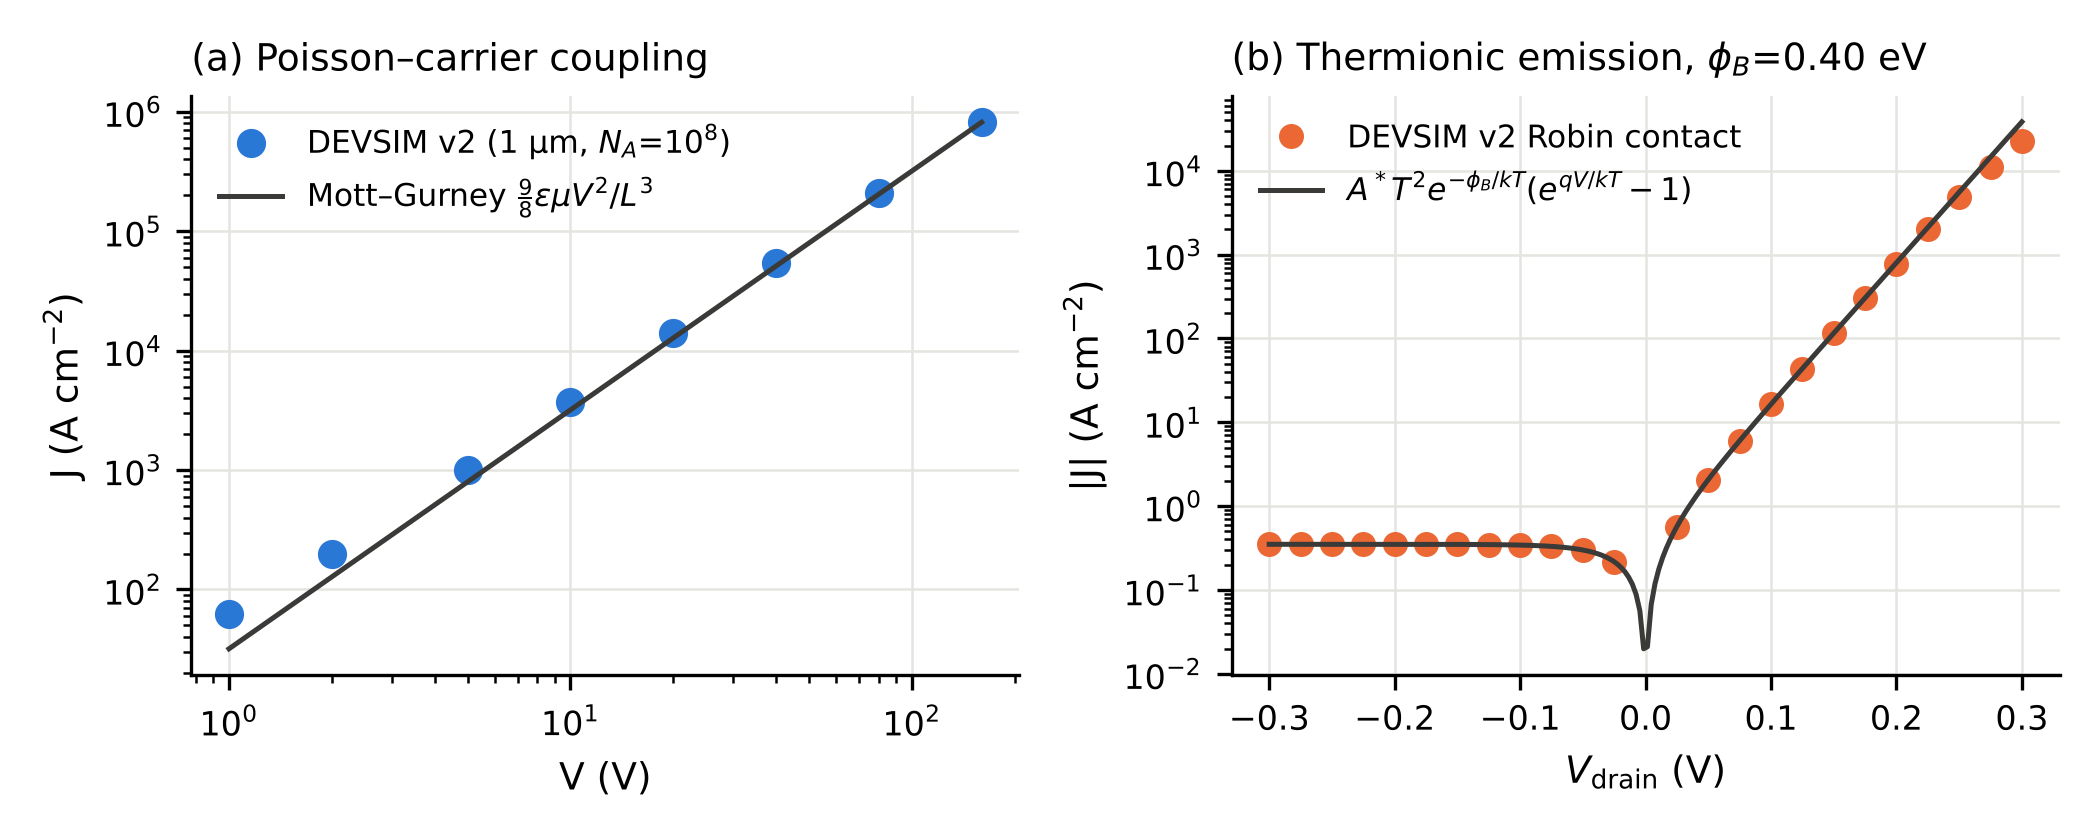
\includegraphics[width=\textwidth]{fig1_verification.png}
\caption{Verification. (a) Mott--Gurney space-charge-limited current in a 1-$\mu$m, nearly intrinsic film with barrier-free contacts. (b) Schottky diode with $\phi_B=0.40$~eV and high mobility compared with thermionic-emission theory.}
\label{fig:verif}
\end{figure}

\section{Results}
\label{sec:results}

\subsection{Work function, pinning and the barrier threshold}
\label{sec:wf}
Figure~\ref{fig:wf}(a) shows the hole barrier used as input. With $S=1$ it falls linearly and reaches zero at $\Phi_M=\chi+E_g=5.0$~eV. $R_{\rm tot}$ [Fig.~\ref{fig:wf}(b)] follows it exponentially, from $1.1\times10^{10}$ (edge) and $4.9\times10^{10}$~\ohmcm\ (top, 50~nm) at 4.33~eV to 11.3 and 15.6~\ohmcm\ at 5.0~eV; a fine sweep (4.90--5.00~eV in 25-meV steps) shows the approach is smooth, with $R_{\rm tot}$ falling by a factor of 4.4 (edge) and 6.2 (top 50~nm) over the last 0.1~eV. Above 5.0~eV the curves are flat only because the barrier is clipped. This threshold is therefore a direct consequence of the adopted Schottky--Mott alignment and the 3.7-eV electron affinity, not an independent prediction. With pinning it moves or disappears: for $S=0.5$ the barrier at 5.0~eV is 0.33~eV and $R_{\rm tot}$(edge) $=1.8\times10^{5}$~\ohmcm, and for $S=0.3$ no metal in the 4.3--5.4~eV range gives a barrier below 0.33~eV (\texttt{pinning\_sweep.csv}). Interface dipoles, metal-induced gap states and thickness-dependent $\chi$ and $E_g$ enter in the same way, through $\Phi_{\rm eff}$ and $E_V$: a 0.1-eV shift of $E_V$ changes $R_{\rm tot}$ at 4.8~eV by a factor of about 25--50 (Fig.~\ref{fig:sens}). We note that the near-ohmic indium electron contacts of Ref.~\cite{refhuang} would correspond, in the same Schottky--Mott picture with $\chi=3.7$~eV, to a 0.6-eV electron barrier, which suggests that interface chemistry or pinning plays a significant role in real InSe contacts; we therefore make no quantitative comparison with that experiment, which also concerns electron rather than hole transport.

\begin{figure}[t]
\centering
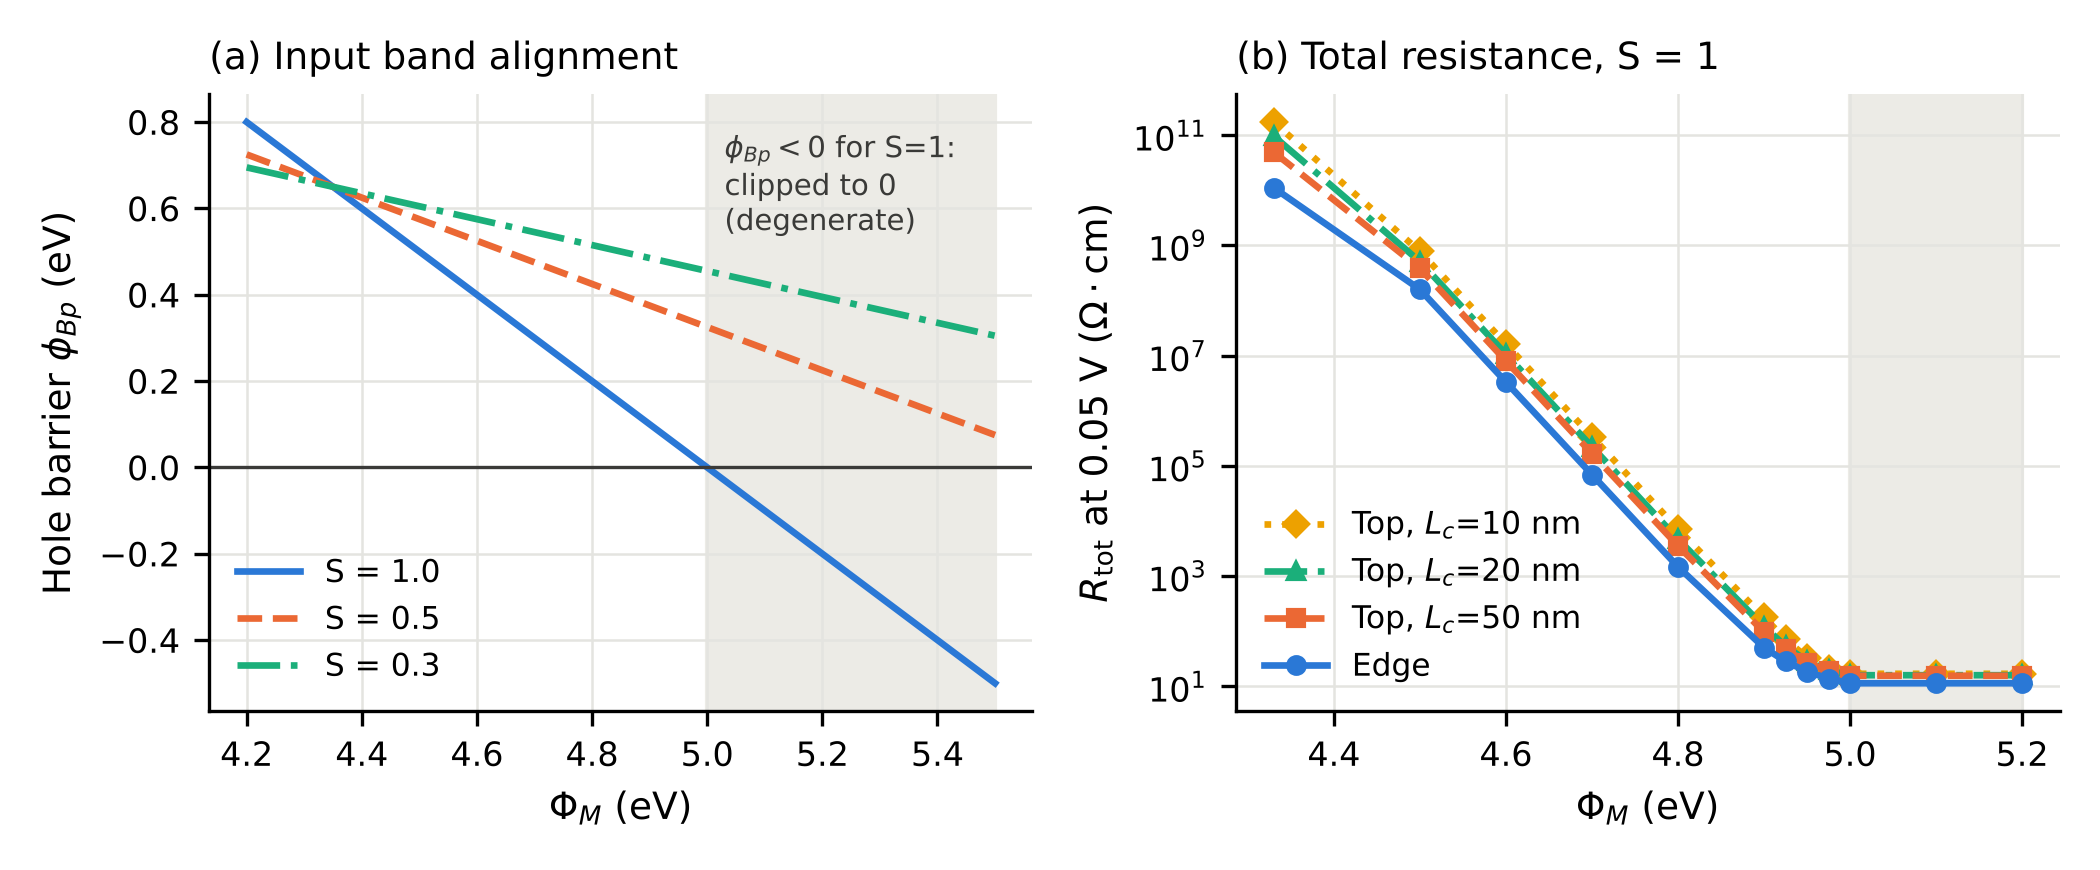
\includegraphics[width=\textwidth]{fig2_barrier_and_resistance_vs_wf.png}
\caption{(a) Hole barrier versus metal work function for pinning factors $S=1$, 0.5 and 0.3. (b) $R_{\rm tot}$ at 0.05~V for top ($L_c=10$, 20, 50~nm) and edge contacts, $S=1$. In the shaded region the Schottky--Mott barrier is negative and has been clipped to zero.}
\label{fig:wf}
\end{figure}

\subsection{Where the resistance is: contact versus channel}
\label{sec:decomp}
Figure~\ref{fig:decomp} decomposes $R_{\rm tot}$. In the barrier-limited case ($\Phi_M=4.8$~eV, $\phi_{Bp}=0.2$~eV) the contacts carry 55--76\% of $R_{\rm tot}$ for top contacts, mostly at the interface itself, and only 7\% for the edge contact. The small edge value does not mean the barrier is unimportant: the 50-nm channel is much shorter than the depletion width at $N_A=10^{16}$~cm$^{-3}$ (about 0.1~$\mu$m for 0.2~eV), so the band bending, and hence the voltage drop, extends across the whole channel and is booked as ``channel''. Shorter top contacts are worse (7130, 4680 and 3530~\ohmcm\ for $L_c=10$, 20 and 50~nm), as expected when the interface conductance per unit length is low. In the barrier-free case ($\Phi_M=5.0$~eV) the channel carries 86--93\% (top) and 99.5\% (edge) of $R_{\rm tot}$; $2R_c=1.17$~\ohmcm\ (top 50~nm) and 0.056~\ohmcm\ (edge). These decomposed contact resistances are independent of $L_{\rm ch}$ across 25--200~nm to within 1\% at 5.0~eV and within 6\% (top) and 12\% (edge) at 4.8~eV (\texttt{lch\_sweep.csv}), which is the expected behaviour of a contact quantity and an internal check of the decomposition. By contrast, a linear transfer-length fit of $R_{\rm tot}(L_{\rm ch})$ gives negative intercepts ($-60$~\ohmcm) at 5.0~eV and, at 4.8~eV, intercepts 1.6 (top) to 10 (edge) times larger than $2R_c$, because $R_{\rm tot}$ is not linear in $L_{\rm ch}$ in either regime [Fig.~\ref{fig:sclc}(c)]. Transfer-length extraction should therefore not be applied to such devices.

\begin{figure}[t]
\centering
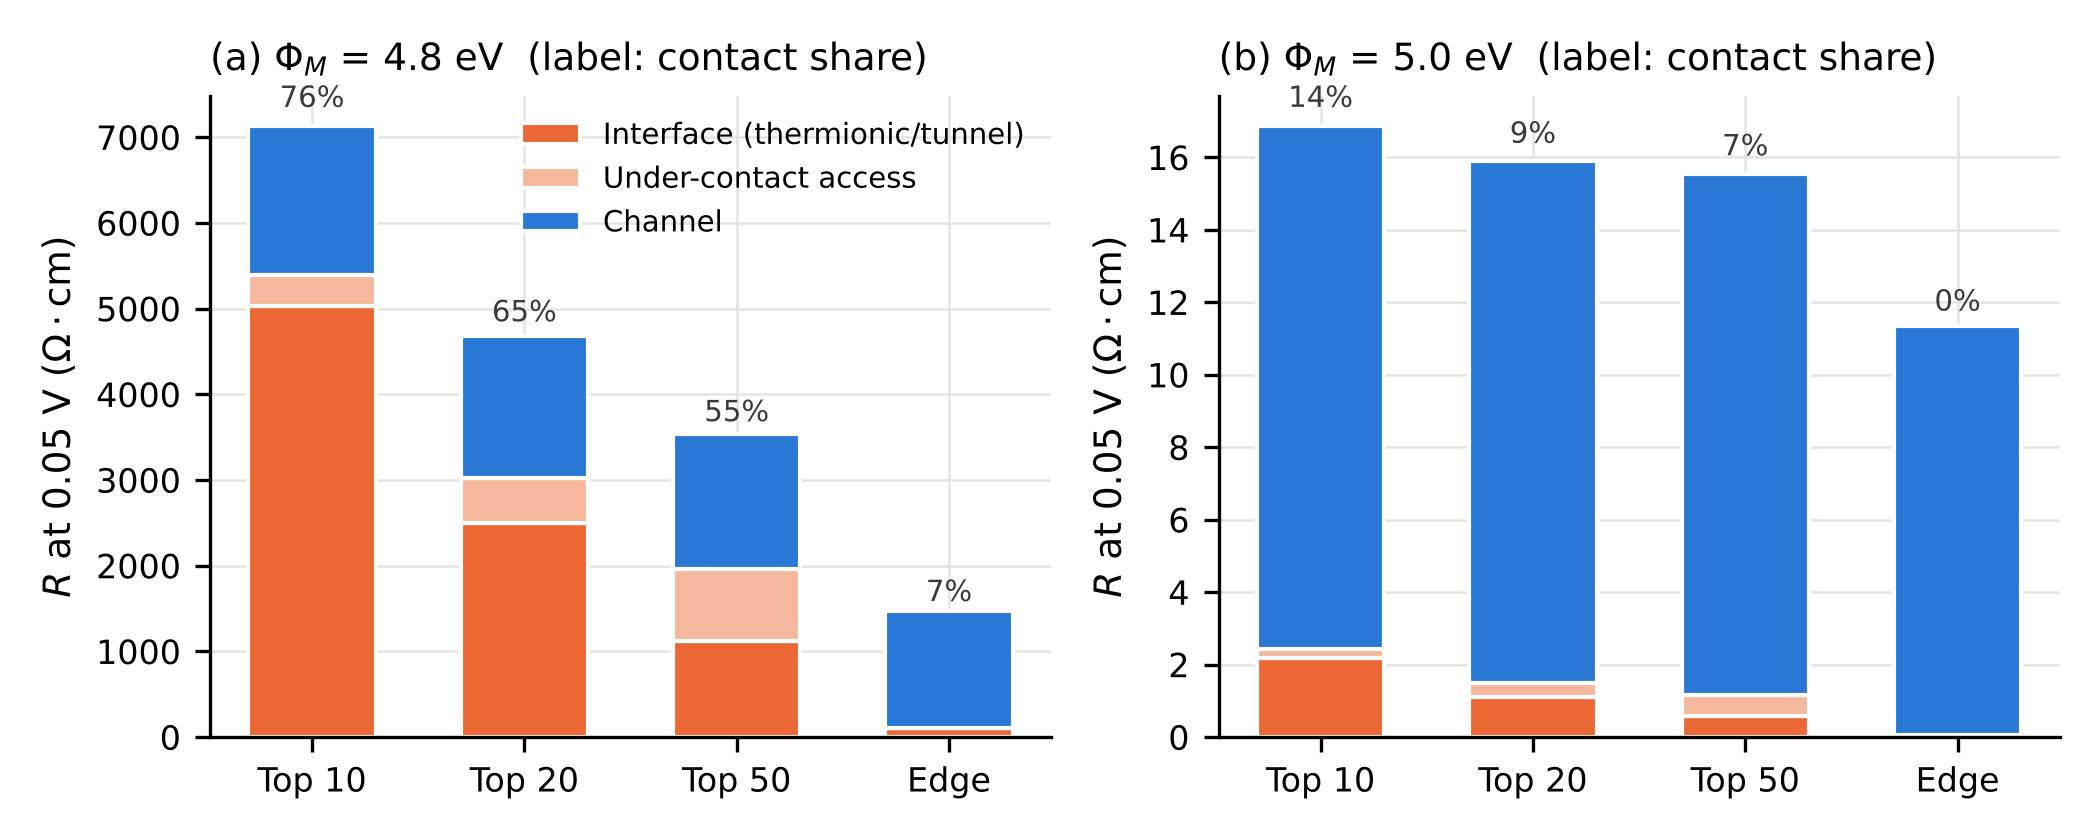
\includegraphics[width=\textwidth]{fig3_resistance_decomposition.png}
\caption{Exact decomposition of $R_{\rm tot}$ at 0.05~V into interface, under-contact access and channel contributions at (a) $\Phi_M=4.8$~eV and (b) 5.0~eV. Labels: contact share $2R_c/R_{\rm tot}$.}
\label{fig:decomp}
\end{figure}

\subsection{Top versus edge: the role of the vdW gap and of tunnelling}
\label{sec:tunnel}
At 0.05~V the edge contact has lower $R_{\rm tot}$ than every top contact at every work function: by 58\% (4.8~eV) and 27\% (5.0~eV) relative to the 50-nm top contact. Figure~\ref{fig:tunnel}(c) shows where this comes from. Removing the vdW gap ($\mathcal{T}_{\rm vdW}=1$) lowers the 50-nm top-contact resistance at 4.8~eV from 3530 to 1540~\ohmcm, within 4\% of the edge value (1480~\ohmcm); widening it to 0.5~nm raises it to $2.4\times10^4$~\ohmcm. At 5.0~eV the gap-free top contact is still 22\% more resistive than the edge contact (14.6 vs 11.3~\ohmcm), a residual geometric effect of the longer access path and smaller injected hole density in the channel. In the barrier-limited regime, then, the top/edge difference is essentially the vdW tunnel barrier, and its magnitude is only as reliable as the assumed $d_{\rm vdW}$ and $\Phi_{\rm vdW}$.

Tunnelling through the Schottky barrier itself is small at this doping. The field-dependent $\Gamma(F)$ lowers $R_{\rm tot}$ by at most 6.1\% (edge, 4.33~eV) and by 2--4\% at 4.6--4.8~eV [Fig.~\ref{fig:tunnel}(a)]; at $N_A=10^{16}$~cm$^{-3}$ the interface field is $\sim10^4$--$10^5$~V/cm and $\Gamma\sim0.2$--2. Because $\Gamma$ now enters a flux condition, it does change the solution when it is large: imposing a constant $\Gamma=100$ (the kind of value the earlier version tested) lowers the 50-nm top-contact resistance at 4.8~eV by 47\% and the edge resistance by 6\% [Fig.~\ref{fig:tunnel}(b)]. The interface velocity therefore matters most where the interface conductance is small, that is, for top contacts with a vdW gap. A nonlocal tunnelling model and heavier doping near the contacts would be needed for quantitative statements about field emission.

\begin{figure}[t]
\centering
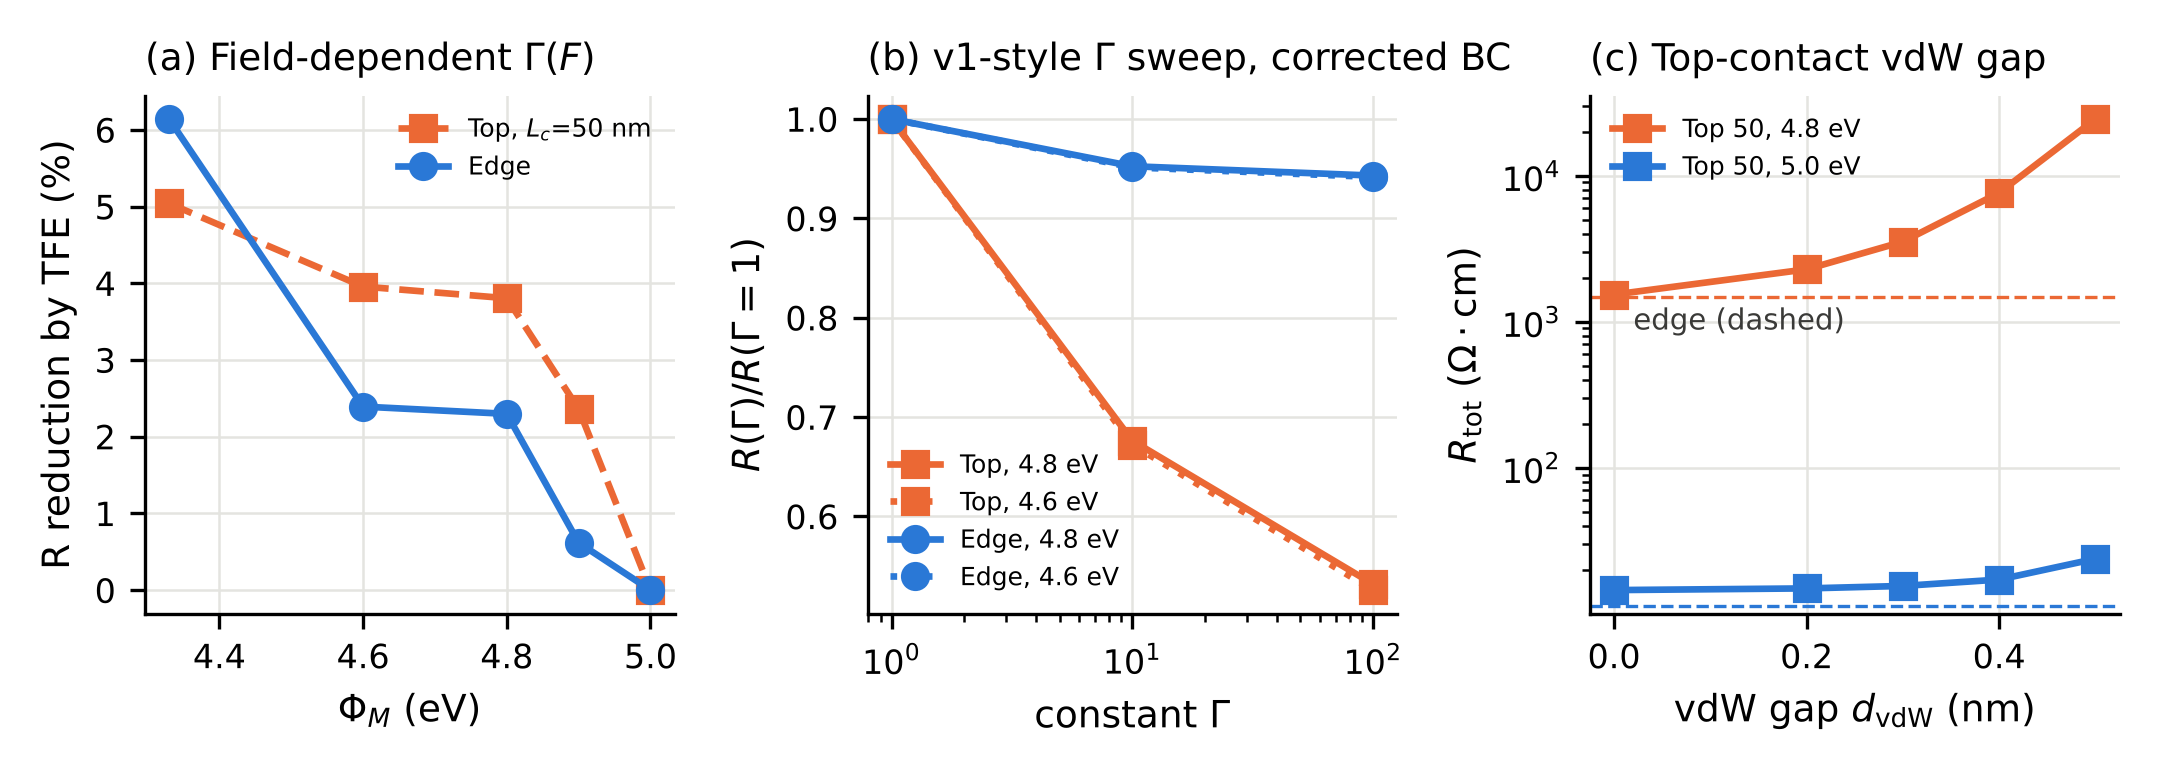
\includegraphics[width=\textwidth]{fig6_tunneling_vdw.png}
\caption{(a) Reduction of $R_{\rm tot}$ by the self-consistent, field-dependent TFE factor $\Gamma(F)$. (b) $R_{\rm tot}$ for an imposed constant $\Gamma$, normalized to $\Gamma=1$, in the corrected flux boundary condition. (c) 50-nm top-contact $R_{\rm tot}$ versus vdW-gap width; dashed lines: edge contact.}
\label{fig:tunnel}
\end{figure}

\subsection{Channel transport in the barrier-free regime}
\label{sec:sclc}
With barrier-free contacts $p_{\rm eq}=N_V=1.76\times10^{18}$~cm$^{-3}$, and holes spill from both contacts into the channel. Even at 0.05~V the centre-line hole density of a 100-nm edge-contacted channel exceeds $N_A$ by a factor of 2.3 at mid-channel and by more than 100 within a few nanometres of the contacts [Fig.~\ref{fig:sclc}(b)]. Consequently $R_{\rm tot}$ scales as $L_{\rm ch}^{2.3}$ (edge) and $L_{\rm ch}^{2.0}$ (top, 50~nm) over 25--200~nm at 0.05~V [Fig.~\ref{fig:sclc}(c)], close to the $L^{-2}$ conductance scaling of space-charge-limited current in thin films \cite{refgrinberg}, whereas at 4.8~eV the length dependence is weak ($L^{0.1}$--$L^{0.3}$) because the barrier, not the channel, controls the current. The bias dependence, however, does not reach a developed space-charge-limited regime. The local exponent $m=d\ln I/d\ln V$ of isothermal edge-contacted devices rises from 1.0 at low bias to a maximum of 1.5--1.7 [Fig.~\ref{fig:sclc}(a)]; power-law fits between 0.4 and 1.2~V give $m=1.47\pm0.02$, $1.44\pm0.02$ and $1.28\pm0.02$ for $L_{\rm ch}=50$, 100 and 200~nm (one standard error of the fit). The 25-nm device instead saturates ($m<1$) as its current approaches the thermionic injection limit $qv_RN_Vt=0.92$~A/cm. We therefore describe the barrier-free channel as contact-injection-dominated, with superlinear I--V and SCLC-like length scaling, but not as a demonstrated Mott--Gurney or thin-film SCLC regime: the exponents are below 2, the background doping is not negligible, and diffusion from both contacts contributes at all biases. Profiles of $p$, $\psi$, $E$ and $\phi_p$ for all cases are provided in \texttt{profiles.npz}.

\begin{figure}[t]
\centering
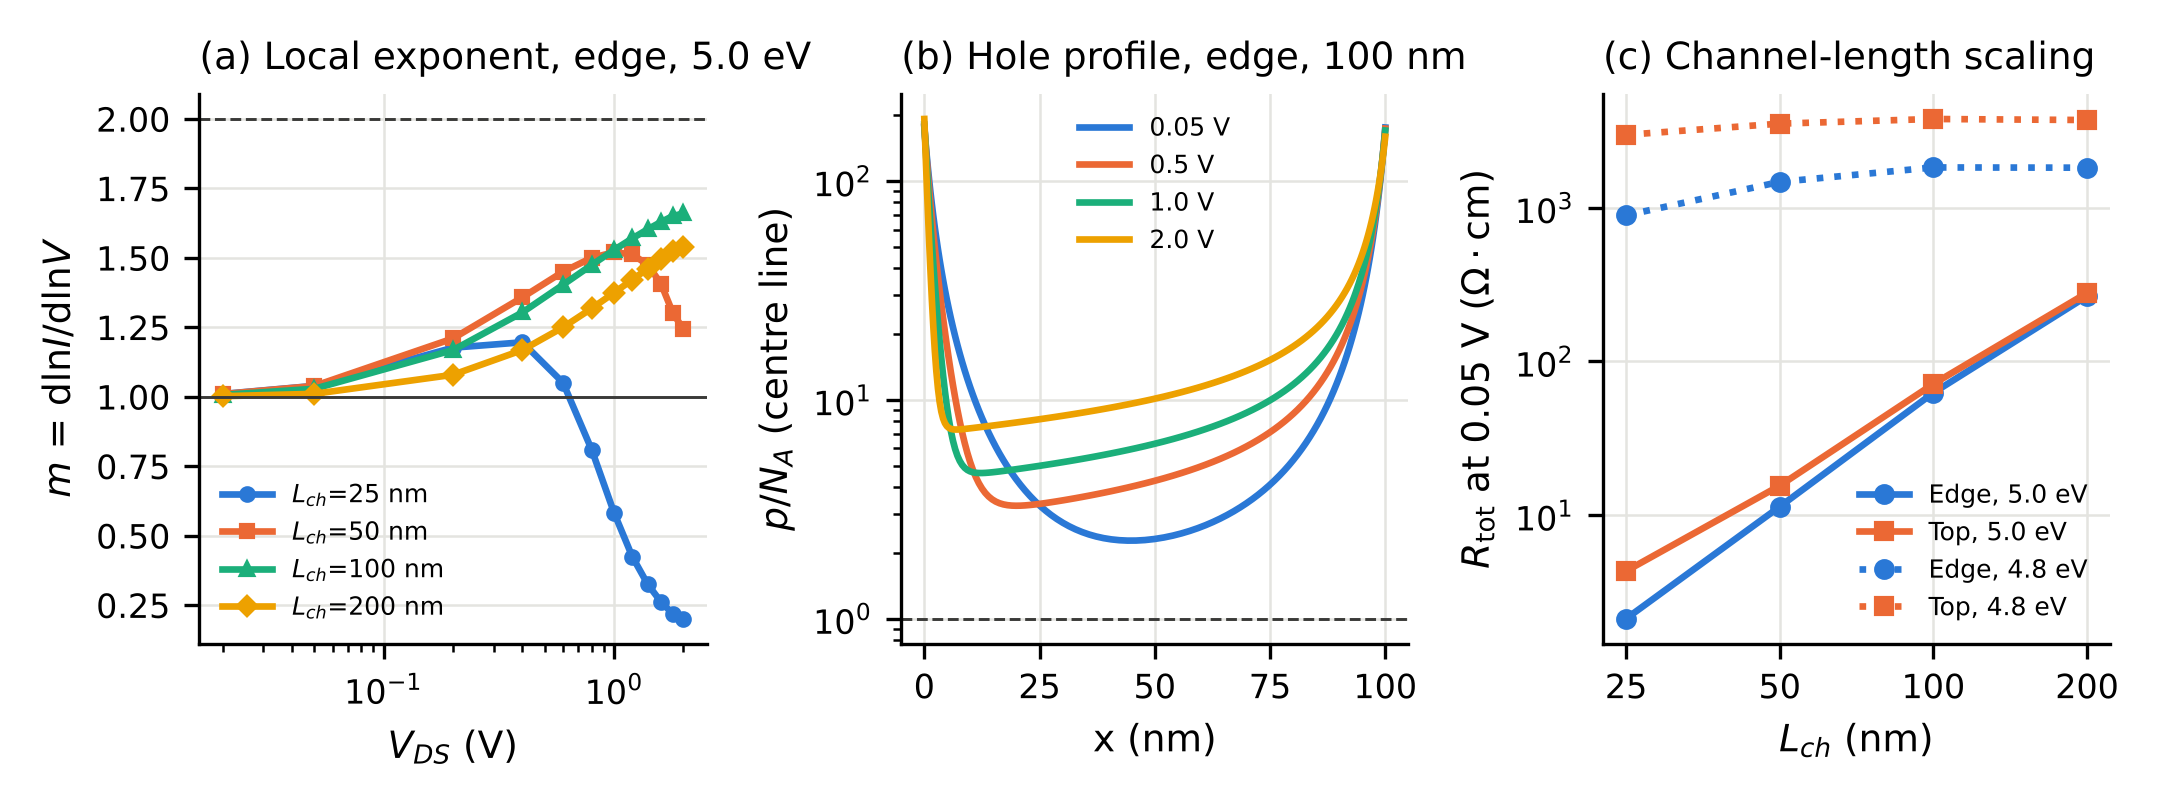
\includegraphics[width=\textwidth]{fig5_sclc_channel_length.png}
\caption{Barrier-free ($\Phi_M=5.0$~eV) channel transport. (a) Local I--V exponent for edge-contacted channels of 25--200~nm (isothermal). (b) Centre-line hole density of a 100-nm edge-contacted channel at 0.05--2~V. (c) $R_{\rm tot}$ at 0.05~V versus channel length at 4.8 and 5.0~eV.}
\label{fig:sclc}
\end{figure}

\subsection{High bias and self-heating}
\label{sec:thermal}
Figure~\ref{fig:iv} and Table~\ref{tab:thermal} compare the geometries at identical operating points. At 5.0~eV the I--V of top contacts saturates: the current approaches the vdW-limited injection capacity $qv_R\mathcal{T}_{\rm vdW}N_VL_c$ (0.024~A/cm for $L_c=10$~nm, approached by 0.5~V; 0.12~A/cm for 50~nm, of which current crowding uses about half), and $dV/dI$ rises to $10^2$--$10^3$~\ohmcm. Edge contacts do not saturate and carry 0.35~A/cm at 2~V, 5.4$\times$ the 50-nm top contact. The resulting temperature rise is larger for the edge contact both at equal bias (105~K vs 7.8~K at 2~V) and at equal dissipated power: the peak rise per unit power is 152~K\,cm/W for the edge contact against 61 (top, 50~nm) and 102~K\,cm/W (top, 10~nm), because the edge-contacted film has a 50-nm thermal footprint on the substrate whereas the top-contacted film also spreads heat under its contacts. Within the model, therefore, edge contacts do not run cooler; their advantage is lower resistance and higher current, and their thermal penalty depends on how heat leaves the device. The peak temperature is set mainly by the substrate heat-transfer coefficient (edge, 2~V: 441~K rise for $h_{\rm sub}$ ten times smaller, 16~K for ten times larger) and by whether metal contacts sink heat (55~K with $h_c=10^4$~W\,cm$^{-2}$K$^{-1}$), and only weakly by $\kappa_{\rm InSe}$ (103--115~K for 0.02--0.2~W/cm\,K); absolute temperatures are therefore model-dependent until $h_{\rm sub}$ and $h_c$ are calibrated for a specific stack. At 4.8~eV self-heating is below 0.3~K up to 2~V for all geometries.

\begin{figure}[t]
\centering
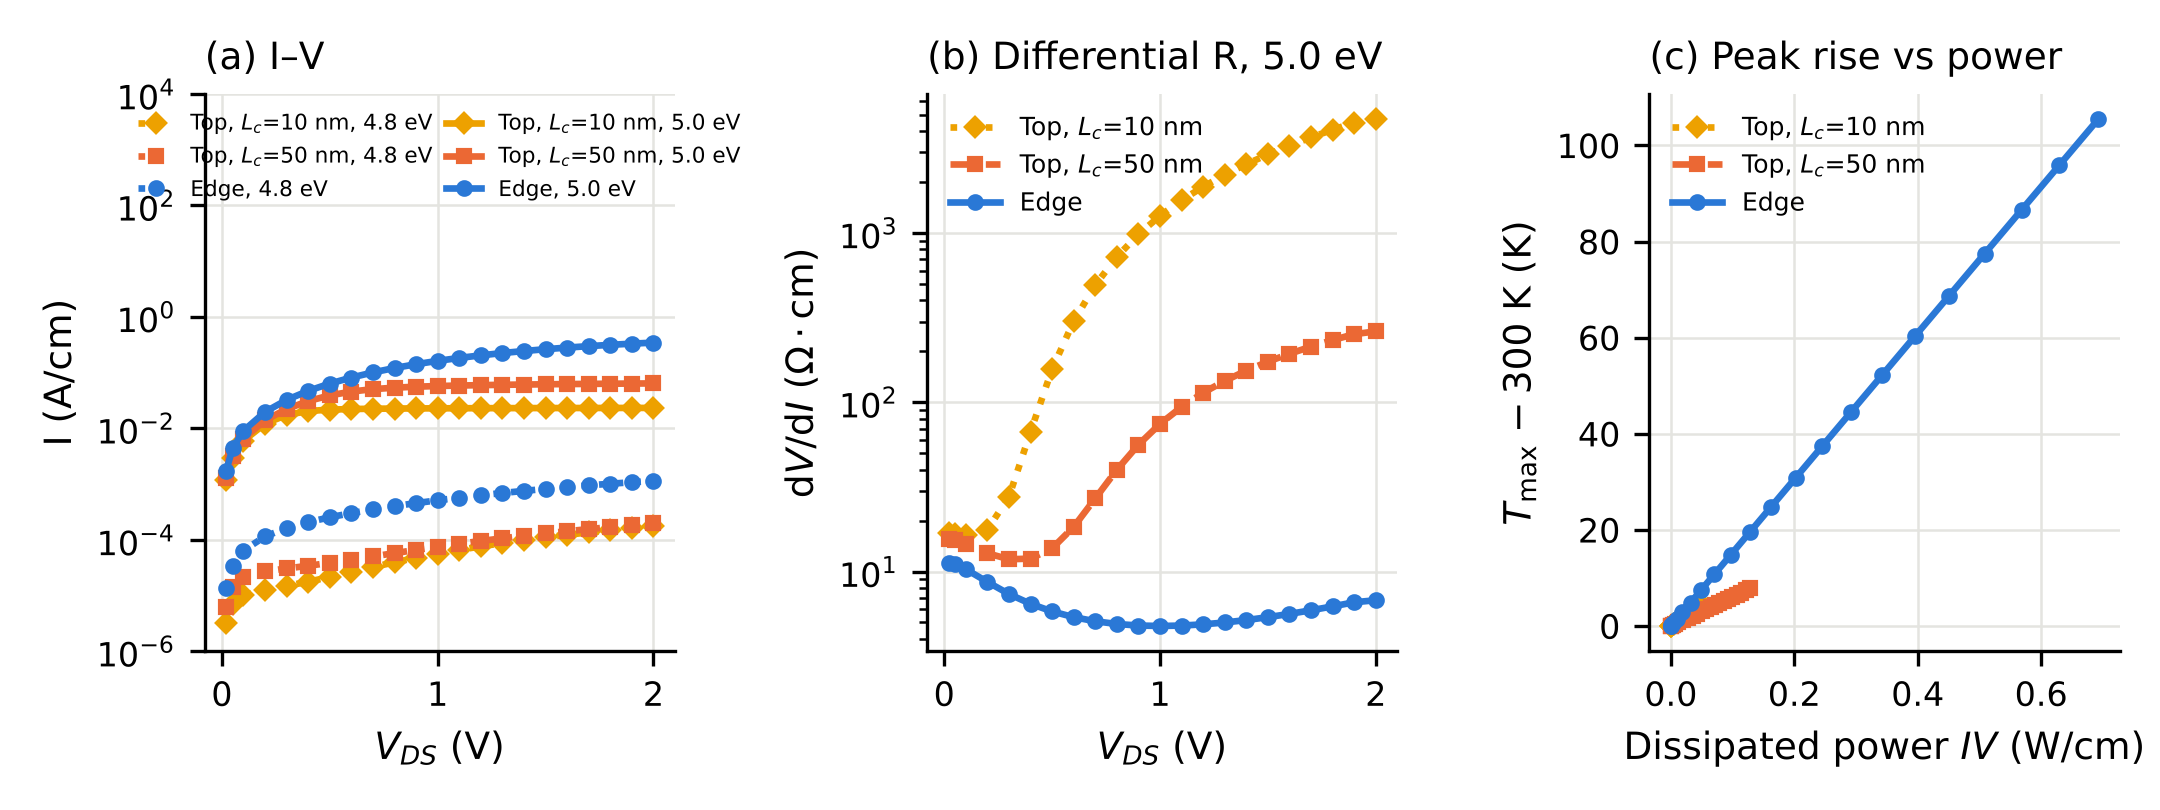
\includegraphics[width=\textwidth]{fig4_electrothermal_iv.png}
\caption{Electro-thermal I--V. (a) Current versus bias at 4.8 (dotted) and 5.0~eV (solid). (b) Differential resistance at 5.0~eV. (c) Peak temperature rise versus dissipated power $IV$ at 5.0~eV.}
\label{fig:iv}
\end{figure}

\begin{table}[t]
\centering
\caption{Operating points at $\Phi_M=5.0$~eV, $L_{\rm ch}=50$~nm, baseline thermal model. All quantities in a row refer to the same bias.}
\label{tab:thermal}
\small
\resizebox{\textwidth}{!}{\begin{tabular}{lcccccc}
\toprule
Geometry & $V_{DS}$ (V) & $I$ (A/cm) & $R_{\rm tot}$ (\ohmcm) & $dV/dI$ (\ohmcm) & $IV$ (W/cm) & $\Delta T_{\max}$ (K) \\
\midrule
Top, 10 nm & 0.05 & 0.00297 & 16.9 & 16.7 & $1.5\times10^{-4}$ & 0.0 \\
Top, 50 nm & 0.05 & 0.00322 & 15.6 & 15.3 & $1.6\times10^{-4}$ & 0.0 \\
Edge & 0.05 & 0.00441 & 11.3 & 11.1 & $2.2\times10^{-4}$ & 0.0 \\
Top, 10 nm & 2.0 & 0.0233 & 85.8 & 4700 & 0.047 & 4.8 \\
Top, 50 nm & 2.0 & 0.0641 & 31.2 & 262 & 0.128 & 7.8 \\
Edge & 2.0 & 0.346 & 5.78 & 6.77 & 0.692 & 105.4 \\
\bottomrule
\end{tabular}}
\end{table}

\begin{figure}[t]
\centering
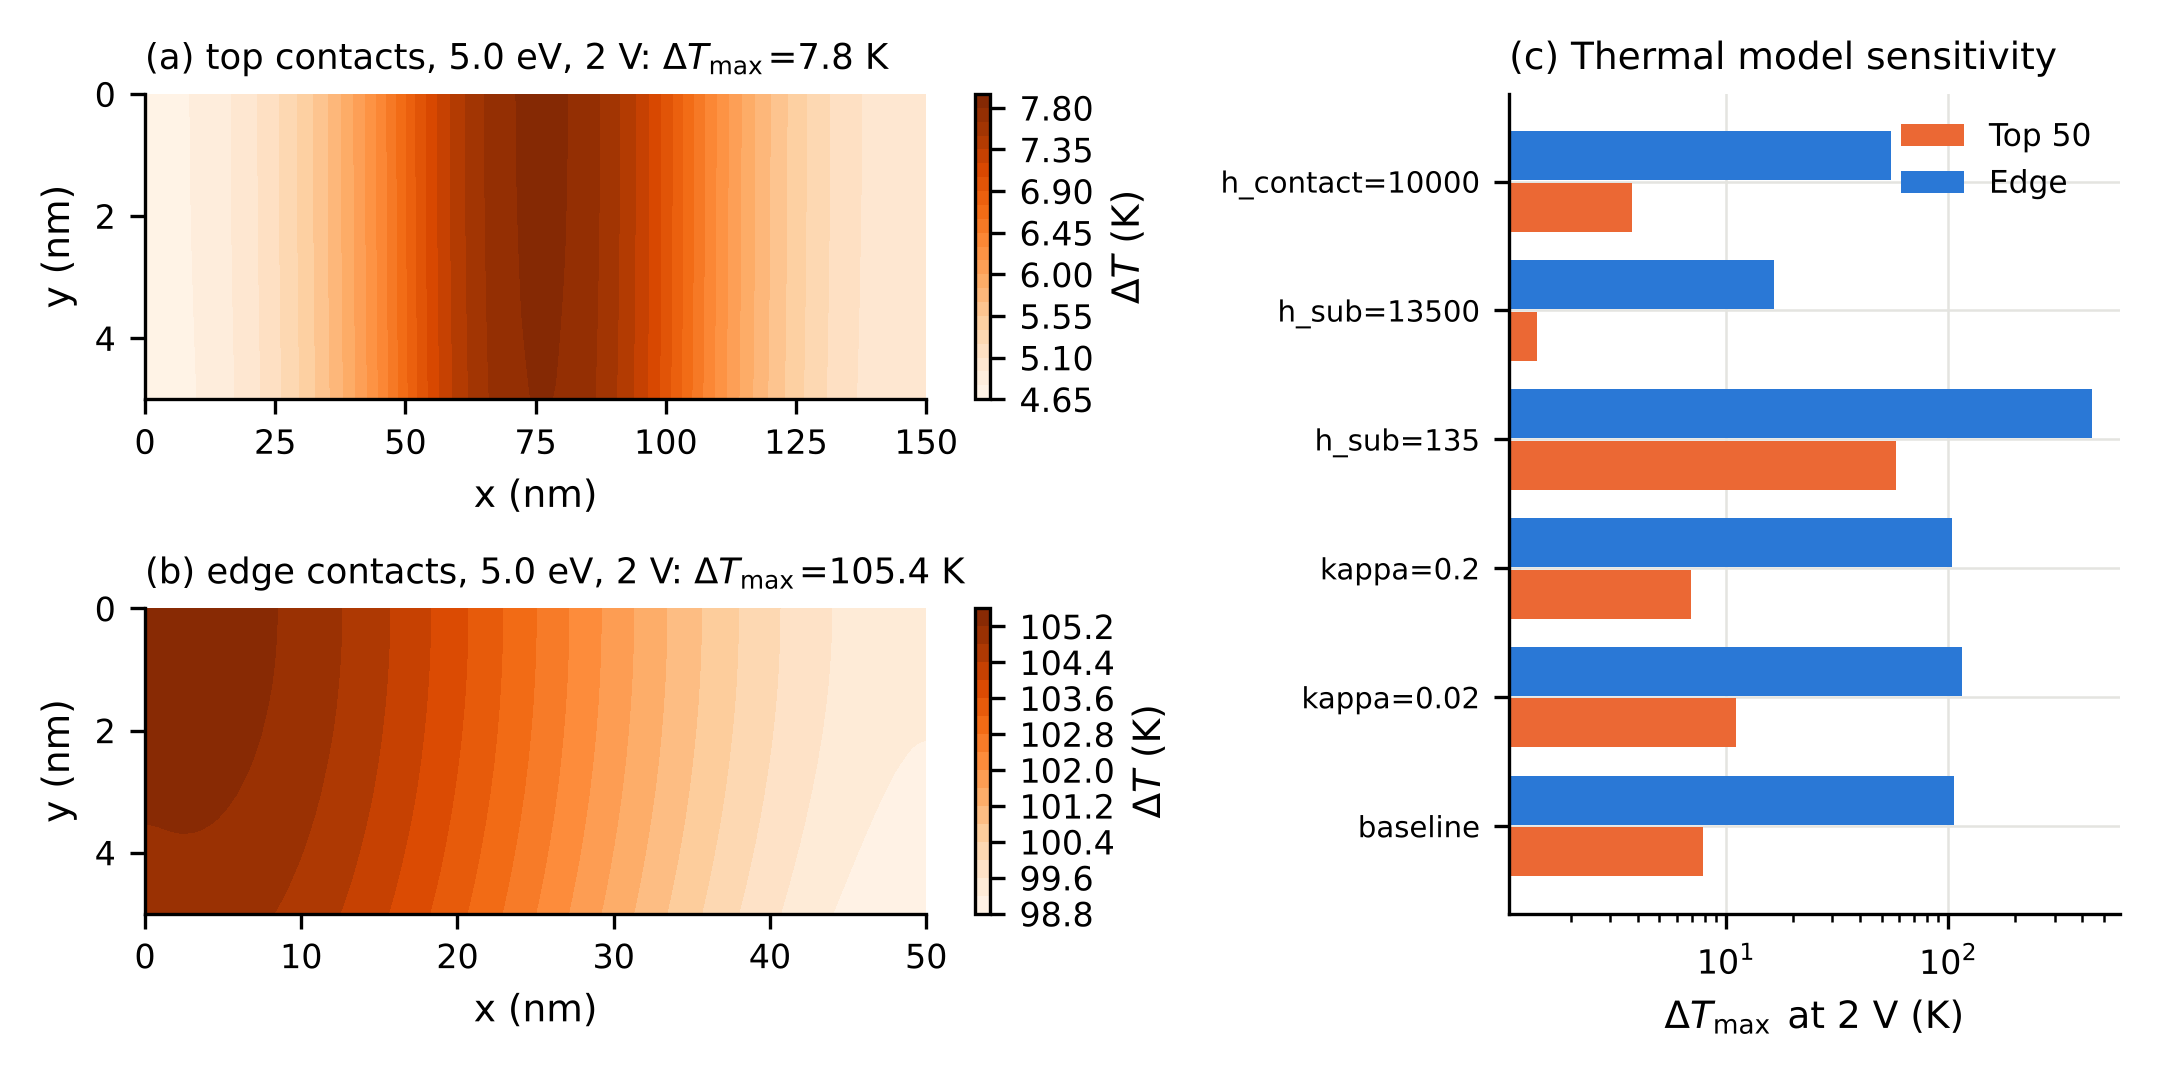
\includegraphics[width=\textwidth]{fig7_thermal.png}
\caption{Lattice temperature rise at 2~V, 5.0~eV for (a) top ($L_c=50$~nm) and (b) edge contacts, and (c) peak rise for variations of $\kappa_{\rm InSe}$ (W/cm\,K), $h_{\rm sub}$ and contact heat sinking $h_c$ (W\,cm$^{-2}$K$^{-1}$).}
\label{fig:thermal}
\end{figure}

\subsection{Parameter sensitivity}
\label{sec:sens}
Figure~\ref{fig:sens} summarizes the change of $R_{\rm tot}$ at 0.05~V when one parameter is varied. In the barrier-limited case the band alignment dominates: $\pm0.1$~eV in $E_V$ changes $R_{\rm tot}$ by factors of 0.04--47, and raising $E_g$ to 1.45~eV at fixed $\chi$ (a plausible value for thinner films) raises it by more than two orders of magnitude. $\mu_p$, $m_h$ and $N_A$ change $R_{\rm tot}$ by factors of about 2--4, and $\varepsilon_r$ by less than 2\%. In the barrier-free case $R_{\rm tot}$ is roughly proportional to $1/\mu_p$, and a 0.15-eV deeper $E_V$ (via $E_g=1.45$~eV) reintroduces a barrier and raises $R_{\rm tot}$ by a factor of 20--35. Background doping is now a moderate parameter (factor $\leq$4 between $10^{15}$ and $10^{17}$~cm$^{-3}$).

\begin{figure}[t]
\centering
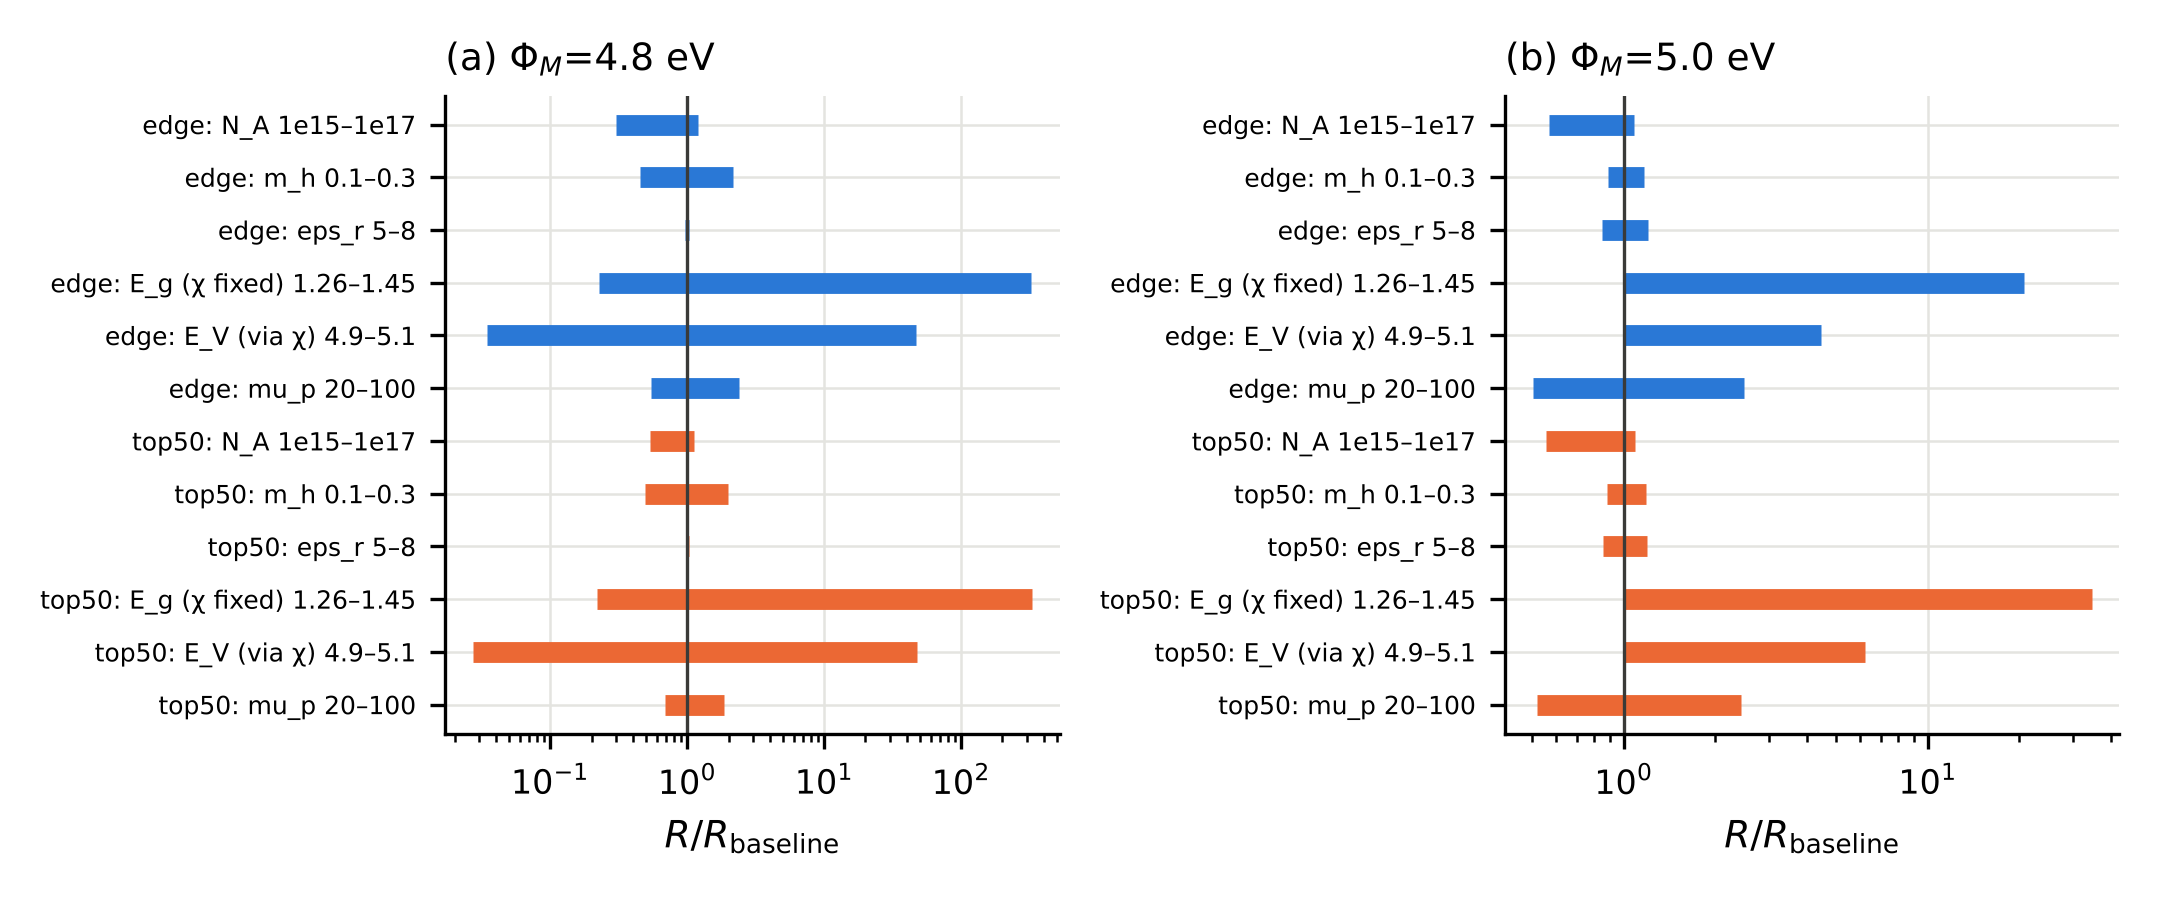
\includegraphics[width=\textwidth]{fig8_parameter_sensitivity.png}
\caption{Range of $R_{\rm tot}/R_{\rm baseline}$ at 0.05~V for one-at-a-time parameter variations at (a) 4.8 and (b) 5.0~eV.}
\label{fig:sens}
\end{figure}

\subsection{Relation to the earlier version of this work}
\label{sec:v1}
The earlier version (repository folder \texttt{src/}) differed in five implementation points, all corrected here: the contact expression $qv(1+\Gamma)(p-p_{\rm eq})$ was used as the residual of a Dirichlet-type contact equation, which enforces $p_s=p_{\rm eq}$ for any nonzero prefactor, so $\Gamma$ and $\mathcal{T}_{\rm vdW}$ could not affect the result; Poisson's equation retained the equilibrium charge after drift-diffusion was enabled; the background was n-type ($+10^{16}$~cm$^{-3}$) instead of p-type; the contact potential carried a sign error in the $\ln(N_C/N_V)$ term; and resistance at 0.1~V was paired with temperature at 2~V. The earlier conclusions that tunnelling is irrelevant because resistance was invariant to $\Gamma$, that the barrier-free channel is SCLC, that the edge advantage is geometric, and that edge contacts run 94~K cooler, do not hold in the corrected model and are withdrawn.

\section{Conclusions}
\label{sec:concl}
For hole injection into a 5-nm InSe channel, the corrected and verified model gives four results. First, the resistance threshold near 5.0~eV is the Schottky--Mott valence-band edge of the input alignment and disappears for pinning factors $S\leq0.5$; contact-metal selection for p-type InSe hinges on the real barrier height, which must come from experiment. Second, for barrier-limited contacts the top-versus-edge difference (58\% at 4.8~eV) is almost entirely the vdW tunnel gap; without it the geometries differ by 4\%. Third, for barrier-free contacts a 50-nm channel, filled by contact-injected holes, carries 86--99.5\% of the resistance and scales superlinearly with length, so contact resistance must be extracted by decomposition rather than by transfer-length fits. Fourth, top contacts become injection-limited at high bias, while edge contacts deliver up to 5.4$\times$ more current and a larger temperature rise per unit power, so edge-contacted InSe benefits most from heat removal through the contacts and substrate. Quantitative predictions for specific metals require measured barrier heights, vdW-gap parameters and thermal boundary conductances.

\section*{Statements and Declarations}
\paragraph{Acknowledgements} Simulations used DEVSIM, an open-source TCAD tool. I thank the anonymous reviewers of an earlier version, whose code-level reading identified the implementation errors corrected here.
\paragraph{Author contributions} H.A.\ designed the study, developed the simulation code, performed all simulations and analyses, and wrote the manuscript.
\paragraph{Funding} This work received no external funding.
\paragraph{Competing interests} The author declares no competing interests.
\paragraph{Data and code availability} Code (\texttt{src\_v2/}: model, verification, studies, figures), all data (\texttt{data\_v2/}) and figures are available at \url{https://github.com/Brukrish2006/InSe-Top-Edge-Contact-Resistace}. The earlier implementation is retained in \texttt{src/} and \texttt{data/} for transparency.

\begin{thebibliography}{99}
\bibitem{refband} D.A.~Bandurin \textit{et al.}, \textit{High electron mobility, quantum Hall effect and anomalous optical response in atomically thin InSe}, Nat.\ Nanotechnol.\ \textbf{12}, 223 (2017), \doi{10.1038/nnano.2016.242}.
\bibitem{refjiang} J.~Jiang, L.~Xu, C.~Qiu and L.-M.~Peng, \textit{Ballistic two-dimensional InSe transistors}, Nature \textbf{616}, 470 (2023), \doi{10.1038/s41586-023-05819-w}.
\bibitem{refqin} B.~Qin \textit{et al.}, \textit{Two-dimensional indium selenide wafers for integrated electronics}, Science \textbf{389}, 299 (2025), \doi{10.1126/science.adu3803}.
\bibitem{refsong} S.~Song, M.A.~Altvater, W.~Lee, H.~Shin, N.~Glavin and D.~Jariwala, \textit{Indium selenides for next-generation low-power computing devices}, Nat.\ Rev.\ Electr.\ Eng.\ (2025), \doi{10.1038/s44287-025-00251-w}.
\bibitem{refhuang} Y.-T.~Huang \textit{et al.}, \textit{High-performance InSe transistors with ohmic contact enabled by nonrectifying-barrier-type indium electrodes}, ACS Appl.\ Mater.\ Interfaces \textbf{10}, 33450 (2018), \doi{10.1021/acsami.8b10576}.
\bibitem{refallain} A.~Allain, J.~Kang, K.~Banerjee and A.~Kis, \textit{Electrical contacts to two-dimensional semiconductors}, Nat.\ Mater.\ \textbf{14}, 1195 (2015), \doi{10.1038/nmat4452}.
\bibitem{refkang} J.~Kang, W.~Liu, D.~Sarkar, D.~Jena and K.~Banerjee, \textit{Computational study of metal contacts to monolayer transition-metal dichalcogenide semiconductors}, Phys.\ Rev.\ X \textbf{4}, 031005 (2014).
\bibitem{refwang} L.~Wang \textit{et al.}, \textit{One-dimensional electrical contact to a two-dimensional material}, Science \textbf{342}, 614 (2013), \doi{10.1126/science.1244358}.
\bibitem{refguim} M.H.D.~Guimar\~aes \textit{et al.}, \textit{Atomically thin ohmic edge contacts between two-dimensional materials}, ACS Nano \textbf{10}, 6392 (2016), \doi{10.1021/acsnano.6b02879}.
\bibitem{refwachutka} G.K.~Wachutka, \textit{Rigorous thermodynamic treatment of heat generation and conduction in semiconductor device modeling}, IEEE Trans.\ Comput.-Aided Des.\ \textbf{9}, 1141 (1990), \doi{10.1109/43.62751}.
\bibitem{refcrowell} C.R.~Crowell and S.M.~Sze, \textit{Current transport in metal-semiconductor barriers}, Solid-State Electron.\ \textbf{9}, 1035 (1966).
\bibitem{refieong} M.~Ieong, P.M.~Solomon, S.E.~Laux, H.-S.P.~Wong and D.~Chidambarrao, \textit{Comparison of raised and Schottky source/drain MOSFETs using a novel tunneling contact model}, IEDM Tech.\ Dig., 733 (1998).
\bibitem{refpad} F.A.~Padovani and R.~Stratton, \textit{Field and thermionic-field emission in Schottky barriers}, Solid-State Electron.\ \textbf{9}, 695 (1966), \doi{10.1016/0038-1101(66)90097-9}.
\bibitem{refmudd} G.W.~Mudd \textit{et al.}, \textit{The direct-to-indirect band gap crossover in two-dimensional van der Waals indium selenide crystals}, Sci.\ Rep.\ \textbf{6}, 39619 (2016), \doi{10.1038/srep39619}.
\bibitem{refguo} Y.~Guo and J.~Robertson, \textit{Band structure, band offsets, substitutional doping, and Schottky barriers of bulk and monolayer InSe}, Phys.\ Rev.\ Mater.\ \textbf{1}, 044004 (2017), \doi{10.1103/PhysRevMaterials.1.044004}.
\bibitem{refmag} S.~Magorrian, V.~Z\'olyomi and V.~Fal'ko, \textit{Electronic and optical properties of two-dimensional InSe from a DFT-parametrized tight-binding model}, Phys.\ Rev.\ B \textbf{94}, 245431 (2016), \doi{10.1103/PhysRevB.94.245431}.
\bibitem{refgrinberg} A.A.~Grinberg, S.~Luryi, M.R.~Pinto and N.L.~Schryer, \textit{Space-charge-limited current in a film}, IEEE Trans.\ Electron Devices \textbf{36}, 1162 (1989), \doi{10.1109/16.24363}.
\bibitem{refmott} N.F.~Mott and R.W.~Gurney, \textit{Electronic Processes in Ionic Crystals}, 2nd ed., Oxford University Press (1940).
\end{thebibliography}

\clearpage
\appendix
\renewcommand{\thefigure}{S\arabic{figure}}
\setcounter{figure}{0}
\section*{Supplementary figure}
\begin{figure}[h]
\centering
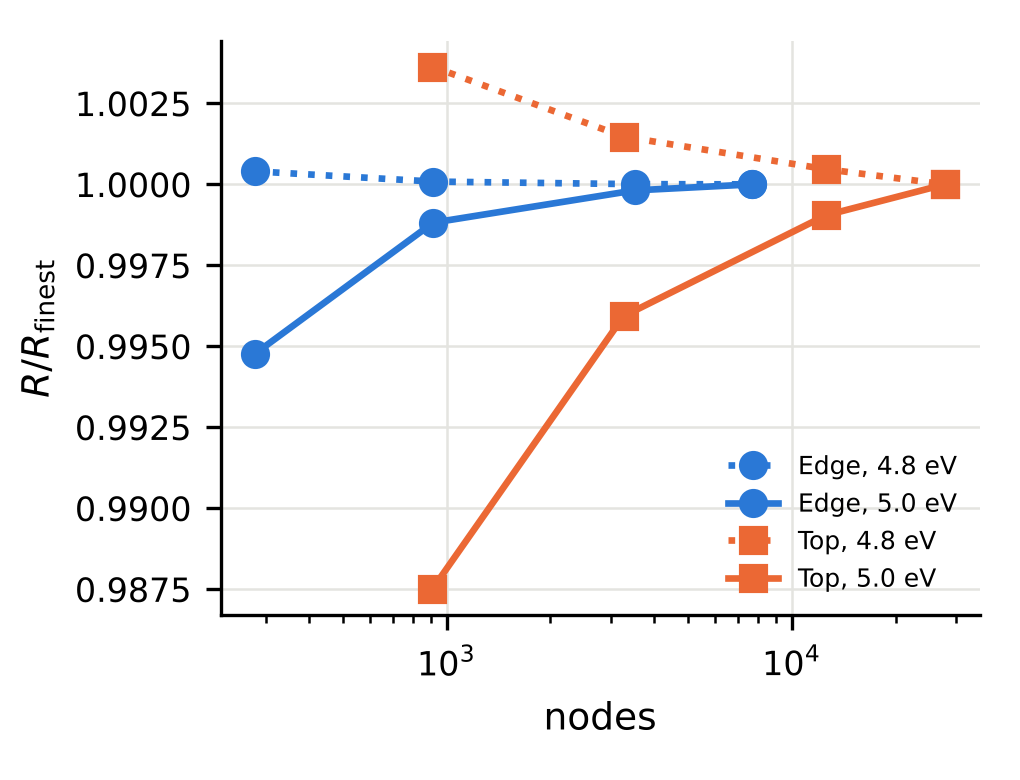
\includegraphics[width=0.5\textwidth]{figS1_mesh_convergence.png}
\caption{Mesh convergence of $R_{\rm tot}$ at 0.05~V (0.5$\times$--3$\times$ density), normalized to the finest mesh.}
\end{figure}

\end{document}
